\chapter{Dynamic Model} \label{ch:model}
A mathematical model of the system needs to be derived in order to simulate and study the effects of nonlinear Geometric Control. In Section \ref{sec:mod.geometric}, an introduction is given about Geometric Mechanics. This is a modern description of the classical mechanics from the perspective of Differential Geometry, which is a discipline in mathematics that studies manifolds and their geometric properties, using the tools of calculus. 

The assumptions that are applied to simplify the model are shortly discussed in Section \ref{sec:mod.assum}. Next, in Section \ref{sec:mod.QRLmod} a dynamical model of the \a{qr}-Load system is obtained with Geometric Mechanics, resulting in a compact, coordinate-free, unambiguous representation of the dynamics, described on nonlinear manifolds.

\section{Geometric Mechanics}\label{sec:mod.geometric}
For the derivation of the equations of motions, traditional modeling methods often parameterize the rotations in a local coordinate system. 
This can be done with Euler Angles, and despite this parametrization might result in singularities, this is a commonly used method to describe rotations. 
There are 24 possible sets of Euler angles and many different conventions are used, which introduces ambiguity. The definition of Euler angles is not unique and a sequence of rotations is not commutative. Therefore, Euler angles are never expressed in terms of the external frame, or in terms of the co-moving rotated body frame, but in a mixture.

Euler angles are kinematically singular since the transformation from their time rates of change to the angular velocity vector is not globally defined. Furthermore, when angular errors are large, the difference in Euler angles is no longer a good metric to define the orientation error. 
%Local coordinates often require symbolic computational tools due to complexity of multi-body systems. 
Hence, the error is rather written as the required rotation to get from the current to a desired orientation, which can be achieved by considering geometric properties of the system.

In Geometric Mechanics the configuration space of systems is a \textit{group manifold} instead of a Euclidean space. The kinetic and potential energies are expressed in terms of this configuration space and their tangent spaces. It explores the geometric structure of a Lagrangian- or Hamiltonian system through the concepts of vector calculus, linear algebra, differential geometry, and nonlinear control theory. Geometric mechanics provides fundamental insights into the nonlinear system mechanics and yields useful tools for dynamics and control theory.

%As a result, the equations of motion and the control systems can be developed on a configuration manifold in a coordinate-free, compact, unambiguous manner, while singularities of local parameterization are avoided.

An example is given of a simple 2-link arm, to illustrate different representations of a configuration space, see Figure \ref{fig:mod.armmanifold}.
Let the configuration of the arm be defined in a Cartesian coordinate system. The position of end-effector $ E $ is  defined as a coordinate in the $ x,y$-plane, which can be calculated with arm lengths $ l_1, l_2 $ and the angles $ \theta_1, \theta_2 $. This can be seen in Figure \ref{fig:mod.armcartesian}. The gray configuration illustrates a singularity, because the definition of one point has multiple solutions.\\
Next, let the configuration be defined by the rotations $ q_1$ and $ q_2$, as shown in Figure \ref{fig:mod.armgeometric}. 
The configuration space is represented as a geometric shape called a \textit{torus}, a smooth manifold where every configuration is mapped uniquely, as shown in Figure \ref{fig:mod.armtorus}. This allows the configuration to be represented globally.
\begin{figure}[h!]
	\centering
	\makebox[.3\textwidth][c]{\subfloat[][\label{fig:mod.armcartesian}]{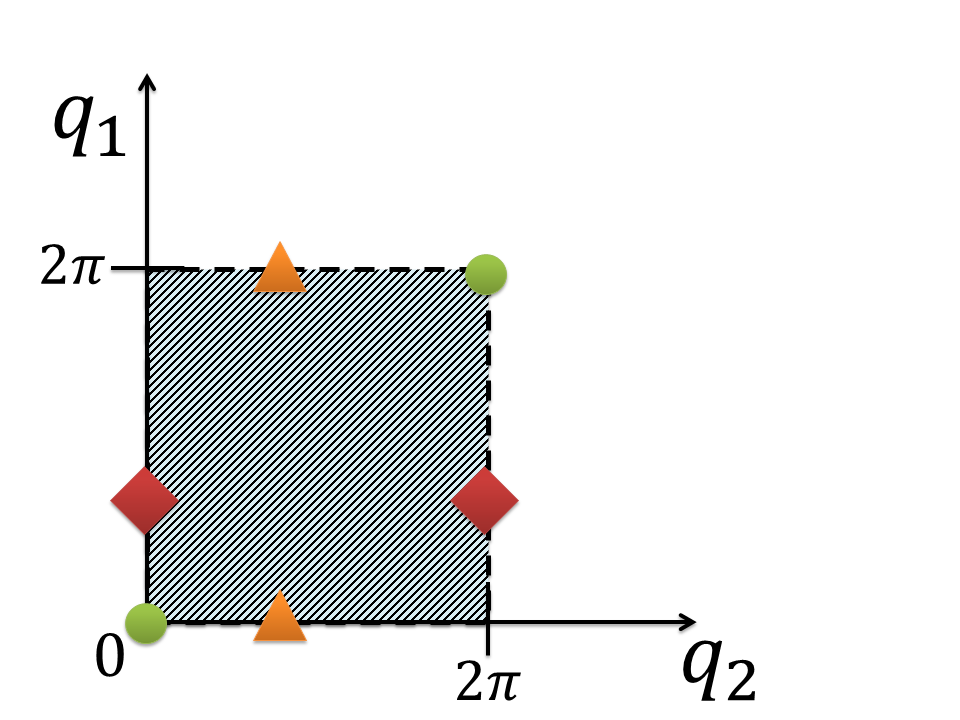
\includegraphics[trim={-3.5cm 0 0 0},clip,width=.35\textwidth]{./StyleStuff/armcartesian.png}}}
	\makebox[.3\textwidth][c]{\subfloat[][\label{fig:mod.armgeometric}]{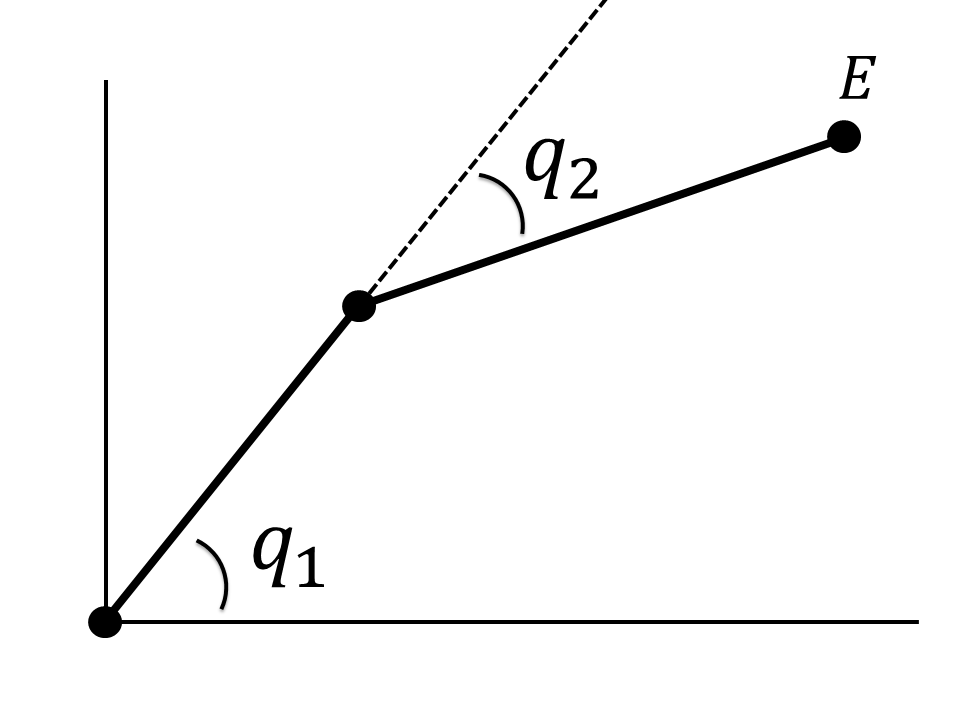
\includegraphics[trim={-3.5cm 0 0 0},clip,width=.35\textwidth]{./StyleStuff/armgeometric.png}}}
	\makebox[.3\textwidth][c]{\subfloat[][\label{fig:mod.armtorus}]{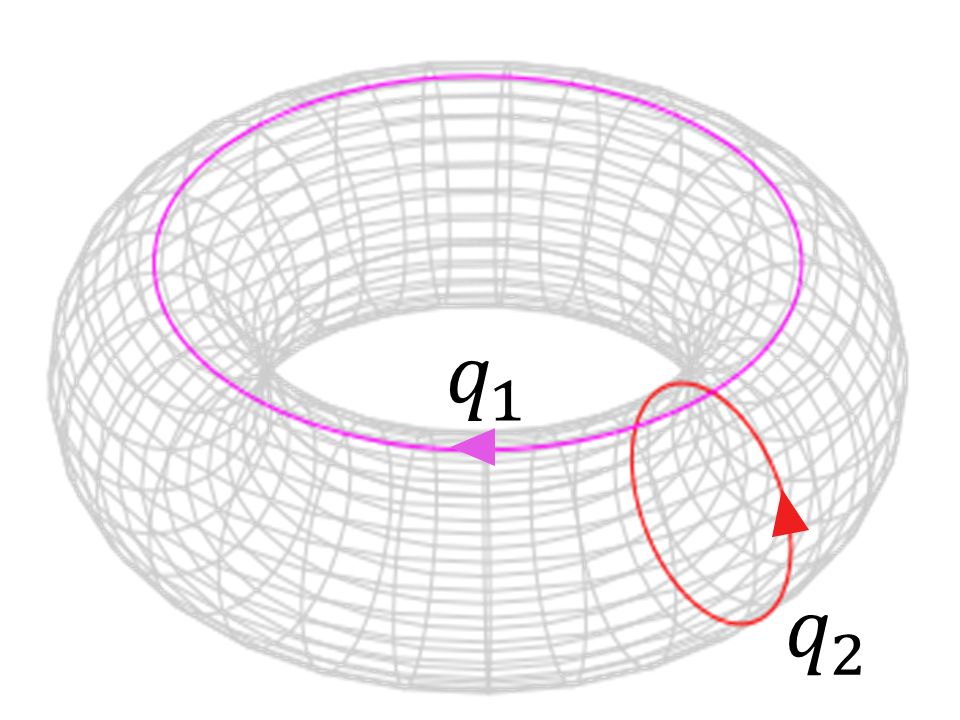
\includegraphics[trim={0 -2.1cm 0 0},clip,width=.30\textwidth]{./StyleStuff/torus.png}}}
	\caption{Configuration Space of a 2-link arm\label{fig:mod.armmanifold}}
\end{figure}		

%CHECK
%Mechanics studies the dynamics of physical bodies acting under forces and potential fields. 
%In Lagrangian mechanics, the trajectories are obtained by finding the paths that minimize the integral of a Lagrangian over time, called the action integral. 
%Rigid body dynamics are characterized by Lagrangian/Hamiltonian dynamics. The dynamics of a Lagrangian system has unique geometric properties and these are exploited to obtain Euler-Lagrange equations. The resulting intrinsic form of the Euler-Lagrange equations are more compact than equations expressed in terms of local coordinates.

\paragraph{Manifolds}
The fundamental object of differential geometry a manifold. A manifold is a mathematical space, a collection of points, that locally resembles Euclidean space near each point. Examples are a plane, a ball, a torus and a sphere. Manifolds are important objects in mathematics and physics because they allow more complicated structures to be expressed and understood in terms of the relatively well-understood properties of simpler spaces. Each point of an n-dimensional manifold has a neighborhood that is homeomorphic to the n-dimensional Euclidean space, meaning that there is a continuous function describing the relation between these spaces, illustrated in Figure \ref{fig:mod.manifold}.
\begin{figure}[h!]
	\centering
	\makebox[\textwidth][c]{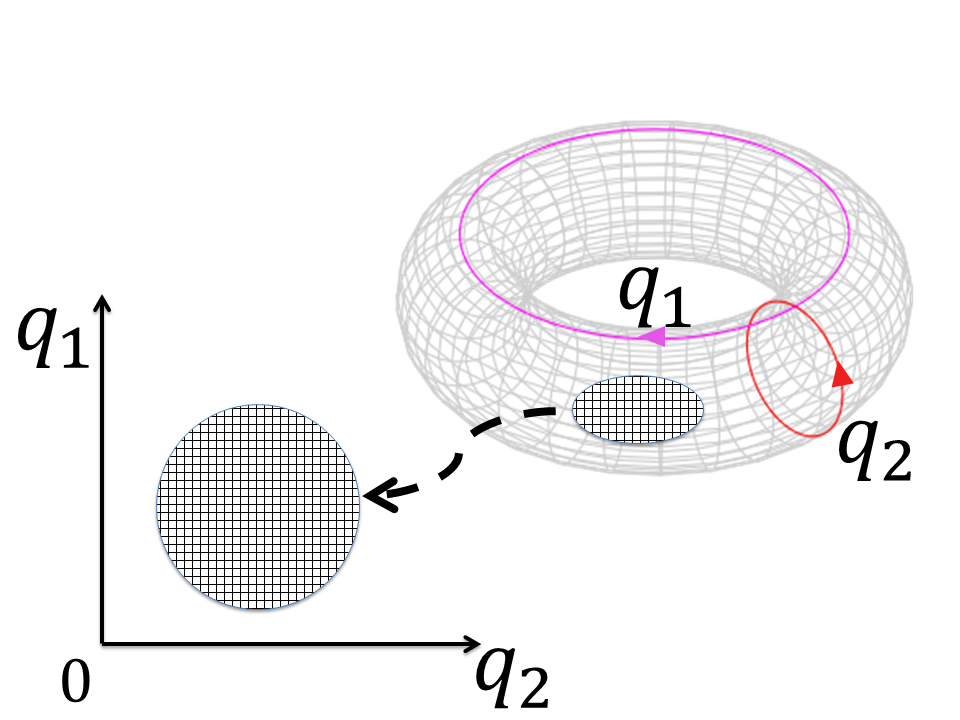
\includegraphics[width=.45\textwidth]{./StyleStuff/manifold.png}}
	\caption{A manifold locally resembles a Euclidean space\label{fig:mod.manifold}}
\end{figure}

%ADD 
%An Introduction to Differentiable Manifolds is given by \cite{Boothby2003}. 
A \textit{differentiable manifold} is a smooth and continuous manifold and is locally similar enough to a linear space to allow to do calculus. One can define directions, tangent spaces, and differentiable functions on such a manifold.\\ 
Taking the derivative at a point on a manifold is equivalent to a \textit{tangent vector} at that point. Meaning that derivatives are conceptually equivalent to an infinitesimally short tangent vector. 
Each point of an n-dimensional differentiable manifold has a tangent space, which is an n-dimensional Euclidean space consisting of all the tangent vectors of all curves that pass through that point. \\
As an example, the manifold $ \mathbb{S}^2 $ is represented as a sphere, with a tangent space at point $ x $, denoted by $ T_x\mathbb{S}^2 $, see Figure \ref{fig:mod.tspace}. 
This illustrates the concept of the relation between $ v $, the derivative of $ x $ in Cartesian space, and the tangent space in on the manifold.
\begin{figure}[h!]
	\centering
	%ADD fig sphere with tangent bundle at x
	\makebox[.49\textwidth][c]{\subfloat[][Representation of a manifold with a tangent space \label{fig:mod.tspace}]{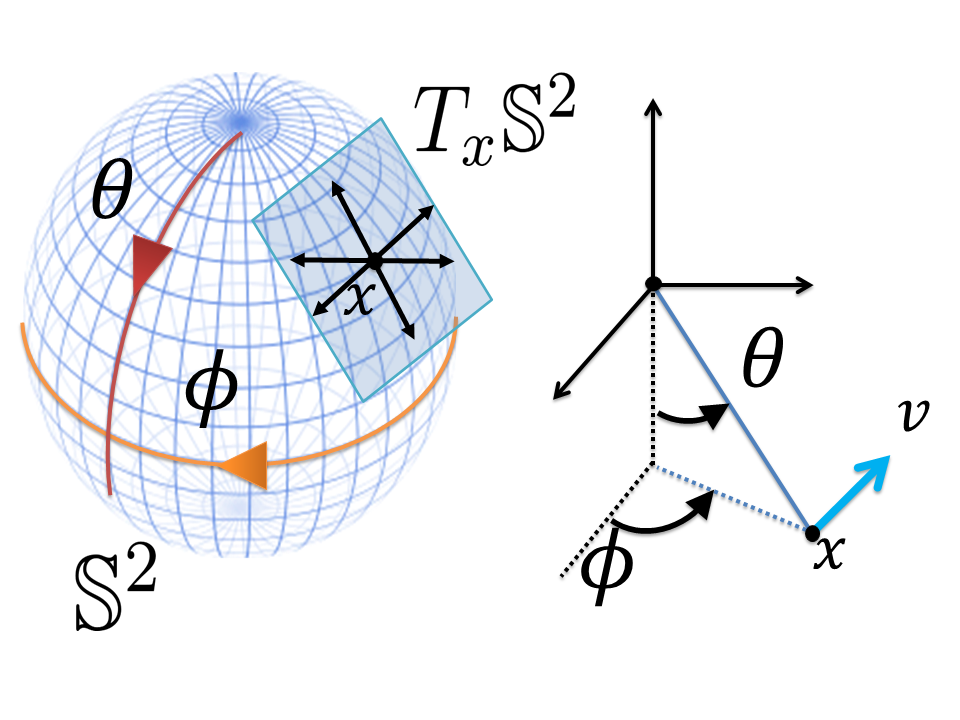
\includegraphics[width=.45\textwidth]{./StyleStuff/tangent.png}}}
	%ADD fig space with SO(3) and so(3)
	\makebox[.49\textwidth][c]{\subfloat[][Identity map of $ SO(3) $ with Lie Algebra $ \mathfrak{so}(3) $ \label{fig:mod.so3}]{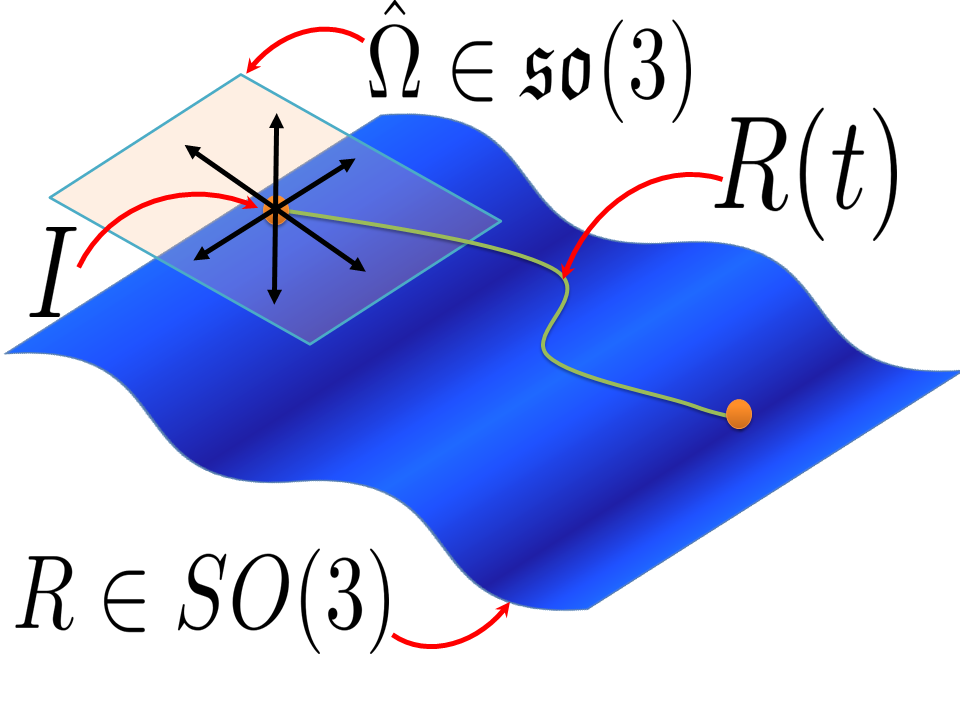
\includegraphics[width=.45\textwidth]{./StyleStuff/so3.png}}}
	\caption{Manifolds and Tangent Spaces\label{fig:}}
\end{figure}		

\subparagraph{Geometric Configuration Spaces}
Several methods exist to describe rotations, such as \textit{Euler Angles}, quaternions or rotation matrices. 
The main disadvantages of Euler angles are that some functions have singularities and they are a less accurate measure for the integration of incremental changes in attitude over time, compared to other methods. 
To avoid these problems, in Geometric Mechanics the rotations are expressed in rotation matrices to provide a global representation of the attitude of a rigid body, by mapping a representation of vectors expressed in \BF to a representation expressed in \IF \cite{Chaturvedi2011,Murray1994}.
 
The configuration of the \a{qr} attitude is expressed in a rotation matrix $ R $ in the Special Orthogonal Group $ SO(3) $ defined as
\begin{equation}\label{eq:SO3}
SO(3) \triangleq \left\lbrace R\in\mathbb{R}^{3\times3}|RR^T=I_{3\times3}, det(R)=1\right\rbrace 
\end{equation}
where $ SO(3) $ is the group of all rotations about the origin of a 3-D Euclidean space, which preserves the origin, Euclidean distance and orientation.

Every rotation has a unique inverse rotation and the identity map satisfies the definition of a rotation. The elements of \textit{Lie Algebra} $ \mathfrak{so}(3) $, a property associated with $ SO(3) $, are the elements of the \textit{tangent space} of $ SO(3) $ at the identity element, see Figure \ref{fig:mod.so3}. 
These elements define the relation between the rotation $ R $ and its derivative $ \dot{R} $, such that
\begin{equation}\label{eq:Rdot}
\dot{R} = R\hat{\Omega}
\end{equation}
For $ n\in \mathbb{N} $, $ \mathfrak{so}(n) $ is is the vector space of skew-symmetric matrices in $ \mathbb{R}^{n\times n} $ and defined as
\begin{equation}\label{eq:so3}
\mathfrak{so}(n) \triangleq \left\lbrace S\in \mathbb{R}^{n\times n}|S^T=-S\right\rbrace
\end{equation}

The hat map $ \wedge:\mathbb{R}^3\rightarrow\mathfrak{so}(3) $ is an isomorphism between $ \mathbb{R}^3 $ and the set of $ 3\times 3 $ skew symmetric matrices, such that $ \hat{x}y=x\times y $ for any $ x,y \in \mathbb{R}^3 $. The vee map $ \vee:\mathfrak{so}(3)\rightarrow\mathbb{R}^3 $, and is the inverse isomorphism of the hat map. Several properties of the hat map are
\begin{eqnarray}
\hat{x}y=x\times y=-y\times x=-\hat{y}x,\\
tr[A\hat{x}]=\frac{1}{2}tr[\hat{x}(A-A^T)]=-x^T(A-A^T)^\vee,\\
\hat{x}A+A^T\hat{x}=(\{tr[A]I_{3\times 3}-A\}x)^\wedge,\\
R\hat{x}R^T=(Rx)^\wedge,
\end{eqnarray}
for any $ x,y\in\mathbb{R}^3, A\in\mathbb{R}^{3\times 3} $, and $ R\in SO(3) $.
The mapping between the body angular velocity vector $ \Omega\in\mathbb{R}^3 $ and  $ \hat{\Omega}\in\mathfrak{so}(3) $ is written as
\begin{equation}\label{eq:mod.hatOmega}
\hat{\Omega}=\begin{bmatrix}
0&-\Omega_3&\Omega_2\\
\Omega_3&0&-\Omega_1\\
-\Omega_2&\Omega_1&0
\end{bmatrix},
\quad
\begin{bmatrix}
0&-\Omega_3&\Omega_2\\
\Omega_3&0&-\Omega_1\\
-\Omega_2&\Omega_1&0
\end{bmatrix}^\vee = \Omega
\end{equation}

The load attitude is expressed as a unit vector $ q $, which points from \BF to the load. The configuration space is a \textit{two-sphere} $\mathbb{S}^2 $ defined as
\begin{equation}\label{key}
\mathbb{S}^2 \triangleq \left\lbrace q\in\mathbb{R}^{3}|q\cdot q=1\right\rbrace 
\end{equation}
The plane tangent to the sphere at $ q $ is the tangent space
\begin{equation}\label{key}
T_q\mathbb{S}^2 \simeq \left\lbrace \omega\in\mathbb{R}^{3}|q\cdot\omega=0\right\rbrace 
\end{equation}

%ADD sphere - tangent space - perpendicular : angular velocity
where $ \omega $ is the angular velocity of the suspended load.
%, such that
%\begin{equation}\label{key}
%\dot{q} = \omega\times q
%\end{equation}


\section{Modeling Assumptions}\label{sec:mod.assum} 

%CHECK intermediate frame. nodig?
The \a{qr} model representation is shown in Figure \ref{fig:mod.model}. Three Cartesian coordinate frames are defined:\v{5}
\begin{itemize}
	\setlength\itemsep{.2pt}
	\item The body-fixed reference frame \lsymb{$ \{\mathcal{B}\} $}{Body Frame} (Body Frame)
	\subitem with unit vectors \lsymb{$ \{\mathbf{b}_1,\mathbf{b}_2,\mathbf{b}_3\} $}{Unit vectors along the axes of $ \{\mathcal{B}\} $} along the axes
	\item The ground-fixed reference frame \lsymb{$ \{\mathcal{I} \}$}{Inertial World Frame} (Inertial Frame)
	\subitem with unit vectors \lsymb{$ \{\mathbf{e}_1,\mathbf{e}_2,\mathbf{e}_3\} $}{Unit vectors along the axes of $ \{\mathcal{I}\} $} along the axes								
	\item The intermediary frame \lsymb{$ \{\mathcal{C} \}$}{Intermediary Frame}, ($ \{\mathcal{I} \}$ rotated by the yaw angle $ \psi $) 
	\subitem with unit vectors \lsymb{$ \{\mathbf{c}_1,\mathbf{c}_2,\mathbf{c}_3\} $}{Unit vectors along the axes of $ \{\mathcal{C}\} $} along the axes								
\end{itemize}

\begin{figure}[h!]
	\centering
	\makebox[\textwidth][c]{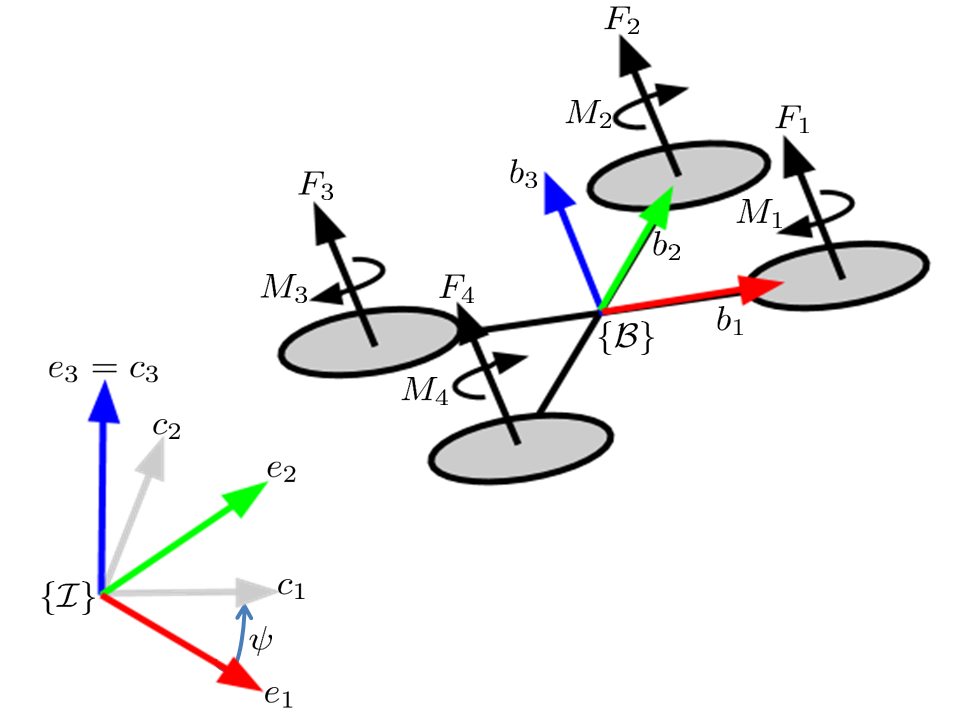
\includegraphics[width=.5\paperwidth]{./StyleStuff/qrmodel.png}}
	\caption{Quadrotor model representation\label{fig:mod.model}}
\end{figure}	



%BART
%***************************************\\
%This is a bit a dead end. I expect something after thsi. FOr example and evaluation of these methods and then the one you are using.
%
%***************************************\\

%CHECK is dit wel nodig?
The complex dynamics of the rotors and their interactions with drag and thrust forces are represented by a simplified model. 
The angular speed \lsymb{$ \omega_i $}{Angular speed of rotor $ i $} of rotor $ i $, for $ i=1,2,3,4 $, generates a force \lsymb{$ F_i $}{Force generated by rotor $ i $} parallel to the direction of the rotor axis of rotor $ i $, given by
\begin{equation}\label{key}
F_i=\left( \frac{K_vK_\tau\sqrt{2\rho A}}{K_t}\omega_i\right)^2\simeq b\omega_i^2 
\end{equation}
where $ K_v,K_t $ are constants related to the motor properties, $ \rho $ is the density of the surrounding air, $ A $ is the area swept out by the rotor, $ K_\tau $ is a constant determined by the blade configuration and parameters, and $ b $ is the thrust factor.\\
The torque around the axis of rotor $ i $, generated due to drag is given by
\begin{equation}\label{key}
M_{i}=\frac{1}{2}R\rho C_DA(\omega_iR)^2\simeq d\omega_i^2
\end{equation}
where $ R $ is the radius of the propeller, $ C_D $ is a dimensionless constant, and $ d $ is the drag constant.

%CHECK directions van de momenten
%CHECK waar is c_tau f gebleven?
The required rotor speeds $ \omega_i $ can be calculated for a given desired total thrust \lsymb{$ f $}{Total thrust. $ f=\sum_{i=1}^{4}F_i $} and total moment \lsymb{$ M $}{Total moment in \BF. $ M=\begin{bmatrix}	M_\phi&M_\theta&M_\psi	\end{bmatrix}^T $}$=\begin{bmatrix}	M_\phi&M_\theta&M_\psi	\end{bmatrix}^T  $, by solving the following equation
\begin{equation}\label{eq:omega_i}
\begin{bmatrix}
f\\M_\phi\\M_\theta\\M_\psi
\end{bmatrix}=
\begin{bmatrix}
b&b&b&b\\
0&-lb&0&lb\\
lb&0&-lb&0\\
-d&d&-d&d\\
\end{bmatrix}
\begin{bmatrix}
\omega_1^2\\
\omega_2^2\\
\omega_3^2\\
\omega_4^2\\
\end{bmatrix}
\end{equation}
where \lsymb{$ l $}{Distance from the rotor to the QR CM} is the distance from the rotor to the \a{qr}'s \a{cm} and $ M_\phi, M_\theta, M_\psi $ denote the moments around the $ x, y, z $-axis in \BF, respectively. 

Table \ref{tab:mod.assumptions} shows the assumptions that are used for modeling the \a{qr}-Load system, simplifying the complexity of the model.

\begin{table}[h!]
	\centering
	\begin{tabular}{|p{\textwidth}|}
		\hline 		\vspace{0.1mm}
		\textbf{Modeling assumptions Quadrotor model}\\ 	\vspace{0.1mm}		
		%		\tabitem The rotation of the Earth does not affect the flight of the \a{qr}\\
		\tabitem The structure of the \a{qr} is rigid and symmetric. \\
		\hspace{4mm} Elastic deformations and shock (sudden accelerations) of the \a{qr} are ignored.\\										
		\tabitem The mass distribution of the \a{qr} is symmetrical in the x-y plane.\\
		\tabitem The inertia matrix is time-invariant.\\
		\tabitem Aerodynamic effects acting on the \a{qr} are neglected.\\
		\hspace{4mm} Blade flapping, Turbulence, Ground Effects.\\
		\tabitem The air density $ \rho $ around the \a{qr} is constant.\\
		%		\hspace{4mm} An indoor environment guarantees the absence of unpredictable disturbances like wind\\ 
		%		\hspace{4mm} gusts. The model complexity decreases without modeling the effects of wind.\\ 	
		\tabitem The propellers are rigid $ \Rightarrow $ The thrust produced by rotor $ i $ is parallel to the axis of rotor $ i $.\\
		\tabitem Drag factor \lsymb{$ d $ }{Drag factor} and thrust factor \lsymb{$ b $}{Thrust factor} are approximated by a constant.\\
		\hspace{4mm} Thrust force $ F_i $ and moment \lsymb{$ M_{i} $}{Drag moment generated by each propellor} of each propeller is proportional to the square of \\
		\hspace{4mm} the propeller speed. \\
		%		Such that $ F_i = b\omega_i^2$ and $ M_{i} = d\omega_i^2$, where \lsymb{$ \omega_i $}{Angular velocity of rotor $ i $ around its axis, $ i=\{1,2,3,4\} $} is the rotor speed.\\
		\hline 		\vspace{0.1mm}		
		\textbf{Modeling assumptions Quadrotor-Load model}\\ 	\vspace{0.1mm}		
		\tabitem The cable is modeled as a rigid and massless cable. \\
		\tabitem The cable is connected to a friction-less joint at the origin of the body-fixed. \\
		\tabitem The tension in the cable is considered to be non-zero.\\
		\hspace{4mm} This implies that the QR-Load subsystem, consisting of a separate \a{qr} and Load\\
		\hspace{4mm} in free fall, is disregarded.\\		 
		\tabitem Aerodynamic effects acting on the load are neglected.\\
		\hspace{4mm} reference frame.\\
		%		\tabitem Assumption \\
		%		\hspace{4mm} Details Assumption 2\\
		\hline
	\end{tabular}
	\caption{Modeling assumptions}
	\label{tab:mod.assumptions}
\end{table}

%\begin{table}[h!]
%	\centering
%	\begin{tabular}{|p{\textwidth}|}
%		\hline
%		\tabitem The cable is modeled as a rigid and massless cable. \\
%		\tabitem The cable is connected to a friction-less joint at the origin of the body-fixed. \\
%		\tabitem The tension in the cable is considered to be non-zero.\\
%		\hspace{4mm} This implies that the QR-Load subsystem, consisting of a separate \a{qr} and Load\\
%		\hspace{4mm} in free fall, is disregarded.\\		 
%		\tabitem Aerodynamic effects acting on the load are neglected.\\
%		\hspace{4mm} reference frame.\\
%		\tabitem Assumption \\
%		\hspace{4mm} Details Assumption 2\\
%		\hline
%	\end{tabular}
%	\caption{Modeling assumptions Quadrotor-Load model}
%	\label{tab:mod.assumptionsQRL}
%\end{table}


\section{Quadrotor-Load Model}	\label{sec:mod.QRLmod}
The Quadrotor-Load model consists of two subsystems, the first where the cable tension is zero, and the second where the cable tension is non-zero.
In this research, the focus is only on the subsystem where the cable tension is non-zero.
The QR-Load model is shown in Figure \ref{fig:mod.modelQRL}, where the unit vector \lsymb{$ q\in\mathbb{S}^2$}{Unit vector from \a{qr} to Load} gives the direction from the \a{qr} to the Load expressed in \BF. The position of the \a{qr} and Load are related by
\begin{equation}\label{eq:mod.xQ2xL}
x_Q=x_L-Lq
\end{equation}
where \lsymb{$ x_Q \in\mathbb{R}^3$}{Position of the \a{qr} CM} is the position of the \a{qr}'s \a{cm}, \lsymb{$ x_L\in\mathbb{R}^3 $}{Position of the load} is the position of the load, and \lsymb{$ L $}{Length of the cable} is the length of the cable.
\begin{figure}[h!]
	\centering
	\makebox[\textwidth][c]{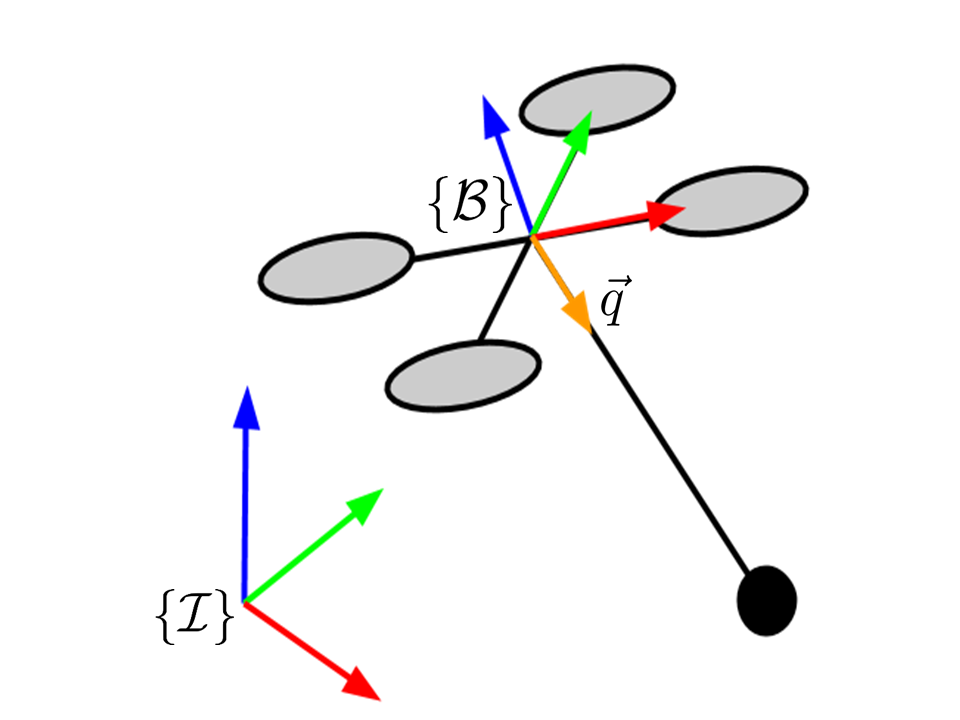
\includegraphics[width=.5\paperwidth]{./StyleStuff/qrlmodel.png}}
	\caption{Quadrotor with Load model representation\label{fig:mod.modelQRL}}
\end{figure}	

Considering the properties of the system, the \a{qr} is described as a rigid body with six degrees of freedom, driven by forces and moments. 
Rigid body dynamics and optimal control problems are studied, and their geometric features are incorporated in \cite{Lee2008}. 
The focus lies on obtaining geometric properties of the dynamics of rigid bodies, how their configuration can be described and how these geometric properties are utilized in control system analysis and design. 

%Which means that the motion of a rigid body can be described by a translation of the \acf{com} and a rotation about the \a{com}. 
%The position of \BF is described by a vector evolving on $ \mathbb{R}^3 $, and is represented with respect to \IF.  

The configuration of the \a{qr} can be described by the location of the \a{qr}s \a{cm}, $x_Q\in \mathbb{R}^3 $, described in the Euclidean space w.r.t. \IF and by the orientation of \BF, also called attitude, w.r.t. \IF evolving on a nonlinear space $R\in SO(3) $.\\
The configuration of the load can be described by its location $x_L\in \mathbb{R}^3 $ w.r.t. \IF, evolving in Euclidean space, and attitude $ q\in \mathbb{S}^2 $ evolving on a nonlinear space called \textit{two-sphere}.\\
%In order to avoid these complexities, 
To conclude, all the dynamics of the \a{qr}-Load system can be globally expressed on the Special Orthogonal Group $SO(3)$, \textit{two-sphere} $ \mathbb{S}^2 $ and Special Euclidean Group $ SE(3) $. This results in a compact notation of the equations of motion, making the large amount of trigonometric functions unnecessary, that Euler angles normally introduce. 

To develop the Euler-Lagrange equations for mechanical systems that evolve on manifolds, an approach developed by \cite{Lee2008,Lee2005,Lee2009,Lee2011} is applied. 
The basic idea is to express the variations of the curves evolving on $ \mathbb{S}^2 $ and $ SO(3) $ in terms of the Lie Algebra $ \mathfrak{so}(3) $, see Equations \ref{eq:mod.var}.  
This approach is based on Hamilton's principle, which states that the evolution of a physical system is a solution of the functional equation given by
\begin{equation}\label{key}
\frac{\delta S}{\delta \mathbf{x}(t)}=0
\end{equation}
%CHECK fact, is that what q defines?
where $ \mathbf{x} $ defines the configuration space. $ S $ is the action integral, defined as
\begin{equation}\label{eq:actionintegral}
S=\int_{t_1}^{t_2}\mathcal{L}dt
\end{equation}
where $\mathcal{L}=\mathcal{T}-\mathcal{U} $ is the Lagrangian of the system, and $\mathcal{T},\mathcal{U}$ are the kinetic and potential energy, respectively. 

%Hamilton's principle requires that the first-order change of  $ \delta S $ is zero for all possible perturbations, meaning that the true path is a stationary point of the action integral, which is defined as
Hamilton's principle of least action states that the path a conservative mechanical system takes between two states $ \mathbf{x}_1 $ and $ \mathbf{x}_2 $ at time $ t_1 $ and $ t_2 $, is the one for which Equation \ref{eq:actionintegral} is a stationary point, resulting in
\begin{equation}\label{eq:HamPr}
\delta S=\int_{t_1}^{t_2}\delta\mathcal{L}dt=0
\end{equation}
where $ \delta\mathcal{L} $ is the variation of the Lagrangian. For systems with non-conservative forces and moments, Equation \ref{eq:HamPr} is extended to
\begin{equation}\label{eq:mod.HamPrNon}
\delta S=\int_{t_1}^{t_2}(\delta W+\delta\mathcal{L})dt=0
\end{equation}
where $ \delta W $ is the virtual work. Equation \ref{eq:mod.HamPrNon} is applied to the QR-Load system, where the configuration manifold is $ \mathbb{R}^3\times \mathbb{S}^2\times SO(3) $. With the following states
\begin{equation}
\textbf{x}= \begin{bmatrix}x_L& \dot{x}_L& q& \omega&R&\Omega
\end{bmatrix}^T
\end{equation}


%\paragraph{Euler-Lagrange} 
%CHECK needed?
%Equation \ref{eq:HamPr} can be satisfied if the following Euler-Lagrange equation holds
%\begin{equation}\label{key}
%\frac{\delta \mathcal{L}}{\delta \mathbf{x}}-\frac{d}{dt}\frac{\delta \mathcal{L}}{\delta \dot{\mathbf{x}}}=0
%\end{equation}
%where the Lagrangian $ \mathcal{L}=\mathcal{T}-\mathcal{U} $.
% that the Lagrangian $\mathcal{L}=\mathcal{T}-\mathcal{U} $. 
The kinetic energy $ \mathcal{T} $ and the potential energy $ \mathcal{U} $ for the system are denoted as
\begin{equation}\label{key}
\begin{aligned}
\mathcal{T}&=\frac{1}{2}m_Q\dot{x}_Q\cdot\dot{x}_Q+\frac{1}{2}m_L\dot{x}_L\cdot\dot{x}_L+\frac{1}{2}\Omega \cdot J\cdot\Omega\\
\mathcal{U}&=m_Qgx_Q\cdot e_3+m_Lgx_L\cdot e_3
\end{aligned}
\end{equation}
where \lsymb{$ J\in\mathbb{R}^{3\times 3} $}{Inertia tensor of \a{qr}} is the inertia tensor of the \a{qr}, and \lsymb{$ g $}{Gravitation constant} is the gravity constant.\\
The energy can be rewritten in terms of $ q $ and $ x_L $, by substituting Equation \ref{eq:mod.xQ2xL}, giving
\begin{align}\label{key}
\mathcal{T}&=\frac{1}{2}(m_Q+m_L)\dot{x}_L\cdot\dot{x}_L -m_QL\dot{x}_L\cdot\dot{q} + \frac{1}{2}m_QL^2\dot{q}\cdot\dot{q}+\frac{1}{2}\Omega \cdot J\cdot\Omega\\
\mathcal{U}&=(m_Q+m_L)gx_L\cdot e_3-m_QgLq\cdot e_3
\end{align}
The variations of $ \mathcal{T} $ and $ \mathcal{U} $ are approximated by a first-order Taylor approximation, which results in
\begin{equation}\label{eq:mod.T}
%ADD
\begin{aligned}
\delta\mathcal{T}&\approx \frac{\partial \mathcal{T}}{\partial\dot{x}_L} \delta\dot{x}_L +\frac{\partial \mathcal{T}}{\partial\dot{q}}\delta\dot{q}+\frac{\partial \mathcal{T}}{\partial\Omega}\delta\Omega\\
&=((m_Q+m_L)\dot{x}_L-m_QL\dot{q})\cdot\delta\dot{x}_L+(-m_QL\dot{x}_L+m_QL^2\dot{q})\cdot\delta\dot{q}+(J\Omega)\cdot\delta\Omega\\
%\end{aligned}
%\end{equation}
%%Substituting the constraint in Equation \ref{eq:mod.xQ2xL} and its derivative into Equation \ref{eq:mod.T} results in
%%\begin{equation}\label{eq:mod.T2}
%%%ADD
%%\delta\mathcal{T}=
%%\end{equation}
%
%\begin{equation}\label{key}
%\begin{aligned}
\delta\mathcal{U}&\approx \frac{\partial \mathcal{U}}{\partial{x}_L} \delta{x}_L +\frac{\partial \mathcal{U}}{\partial{q}}\delta{q}\\
&=((m_Q+m_L)ge_3)\cdot\delta x_L-(m_QgLe_3)\cdot\delta q
\end{aligned}
\end{equation}

The first term of virtual work is obtained from $ f $ acting on the \a{qr} and is given by the following term,
\begin{equation}\label{key}
%ADD
\begin{aligned}
\delta W_1&=fRe_3\cdot \sum_{j=1}^{3}\frac{\partial x_Q}{\partial \mathbf{q}_j}\delta \mathbf{q}_j\\
&=fRe_3\cdot(\delta x_L-L\delta q)
\end{aligned}
\end{equation}
where $ \mathbf{q}_j={x_L,q,R} $ and $ x_Q $ is substituted by Equation \ref{eq:mod.xQ2xL}.
The second term of virtual work is obtained from $ M $ acting on the \a{qr}. This gives the following term
\begin{equation}\label{key}
\begin{aligned}
\delta W_2&=M\cdot \sum_{j=1}^{3}\frac{\partial\Omega}{\partial \mathbf{\dot{q}}_j}\delta \mathbf{\dot{q}}_j\\
&=M\cdot(R^T\delta R)
\end{aligned}\end{equation}
The variations in energy and the virtual work can be substituted into Equation \ref{eq:mod.HamPrNon}, such that
\begin{equation}\label{eq:Sfinal}
\delta S = \int_{t_1}^{t_2}(\delta W_1+\delta W_2+\delta\mathcal{T}-\delta\mathcal{U})dt
\end{equation}
While $ x_L,\dot{x}_L $ vary on $ \mathbb{R}^3 $, Equation \ref{eq:Sfinal} is also a function of variations on manifolds, where $ \delta R $ is a variation on $ SO(3) $ and $ \delta q $ is a variation on $ \mathbb{S}^2 $. These so called infinitesimal variations are obtained required as shown in  \cite{Lee2005,Lee2011,Bullo2005,Sreenath2013c}. 
\begin{equation}\label{key}
\begin{aligned}
\delta R&=R\hat{\eta}\in T_RSO(3)&\text{, where } \eta\in\mathbb{R}^3,\hat{\eta}\in\mathfrak{so}(3)\\
\delta q&=\xi\times q \in T_q\mathbb{S}^2&\text{, where }\xi\in\mathbb{R}^3,\xi\cdot q=0
\end{aligned}
\end{equation}
The following variations follow from differentiation,
\begin{equation}\label{eq:mod.var}
\begin{aligned}
\delta \dot{q}&=\dot{\xi}\times q+\xi\times\dot{q},\\
\delta \dot{R}&=\dot{R}\hat{\eta}+R\hat{\dot{\eta}},\\
\delta \hat{\Omega}&=\delta(R^T\dot{R})\\
&=\delta R^T\dot{R}+R^T\delta\dot{R}\\
&=(R\hat{\eta})^T\dot{R}+R^T (\dot{R}\hat{\eta}+R\hat{\dot{\eta}})\\
&=\hat{\eta}^T\hat{\Omega}+\hat{\Omega}\hat{\eta}+\hat{\dot{\eta}}\\
&=({\hat{\Omega}\eta})^\wedge+\hat{\dot{\eta}},\\
\delta\Omega&=({\hat{\Omega}\eta})+{\dot{\eta}}
\end{aligned}
\end{equation}

%CHECK nodig?
%***************************************\\
%Rigid Body Attitude Dynamics evolve on $ SE(3) $.
%\begin{align}\label{eq:eomrigidbody}
%%CHECK waar komt deze equation vandaan?
%J\dot{\Omega}+\Omega\times J\Omega &= mg\rho\times R^Te_3+u\\ 
%\dot{R} &= R\hat{\Omega}
%\end{align}
%***************************************\\

%CHECK standard newton euler
%***************************************\\
%The equations of motion for a rigid body with configuration $ SE(3) $ are given by the \textit{Newton-Euler equations} \cite{Murray1994}:
%\begin{equation}\label{key}
%\begin{bmatrix}
%	mI&0\\
%	0&\mathcal{I}
%\end{bmatrix}
%\begin{bmatrix}
%	\dot{v}^b\\
%	\dot{\omega}^b
%\end{bmatrix}+
%\begin{bmatrix}
%	\omega^b\times mv^b\\
%	\omega^b\times\mathcal{I}\omega^b
%\end{bmatrix}=F^b
%\end{equation}
%where $ m $ is the mass of the body, $ \mathcal{I} $ is the inertia tensor, and $ V^b=(v^b,\omega^b) $ and $ F^b $ represent the instantaneous body velocity and applied body wrench.
%***************************************\\

%ADD equations of motion
%ADD From .... follows
These variations are substituted into Equation \ref{eq:Sfinal}, allowing it to be a function of variations in each generalized coordinate.
\begin{equation}\label{eq:Sfinalfilled}
\begin{aligned}
\delta S &= \int_{t_1}^{t_2}(\delta W_1+\delta W_2+\delta\mathcal{T}-\delta\mathcal{U})dt\\
=&\int_{t_1}^{t_2}(((m_Q+m_L)\dot{x}_L-m_QL\dot{q})\cdot\delta\dot{x}_L+(fRe_3-(m_Q+m_L)ge_3)\cdot\delta x_L)dt\\
&\int_{t_1}^{t_2}((m_QL^2\dot{q}-m_QL\dot{x}_L)\cdot\delta\dot{q}+(m_QgLe_3-fLRe_3)\cdot\delta q)dt\\
&\int_{t_1}^{t_2}(\Omega^TJ \cdot \delta\Omega+M\cdot(R^T\delta R))dt
\end{aligned}
\end{equation}
After rearranging and setting each variation to 0, the following equations of motion for the \a{qr}-Load system are found.
%\begin{eqnarray}\label{eq:mod.eom}
\begin{align}
\frac{d}{dt} x_L &=\dot{x}_L\\
(m_Q+m_L)(\ddot{x}_L+ge_3)&=(q\cdot fRe_3-m_QL(\dot{q}\cdot\dot{q}))q\\
\dot{q}&=\omega\times q\\
m_QL\dot{\omega}&=-q\times fRe_3\\ \label{eq:mod.R}
J\dot{\Omega}+\Omega\times J\Omega&= M\\ \label{eq:mod.attitude}
\dot{R}&=R\hat{\Omega}
\end{align}
%\end{eqnarray}
%\begin{equation}\label{key}
%\hat{\Omega}=\begin{bmatrix}
%0&-\Omega_3&\Omega_2\\
%\Omega_3&0&-\Omega_1\\
%-\Omega_2&\Omega_1&0
%\end{bmatrix}
%\end{equation}

\section*{Summary}
In this chapter, the dynamical model of the Quadrotor-Load system was derived.
%using a Geometric Mechanics modeling approach.
The motivation to use Geometric Mechanics and a basic understanding of its concepts are given in order to understand the difference between a Nonlinear Geometric model and a model obtained with classical modeling approaches.

With the tools of differential geometry, the system dynamics are expressed on nonlinear configuration manifolds, which results in a globally defined, compact, unambiguous representation of the model. This dynamical model is used for a nonlinear geometric control approach, which is discussed in the next chapter.
